\documentclass[12pt]{article}
\usepackage[english]{babel}
\usepackage{natbib}
\usepackage{url}
\usepackage[utf8x]{inputenc}
\usepackage{amsmath}
\usepackage{graphicx}
\graphicspath{{images/}}
\usepackage{parskip}
\usepackage{fancyhdr}
\usepackage{vmargin}
\setmarginsrb{3 cm}{2.5 cm}{3 cm}{2.5 cm}{1 cm}{1.5 cm}{1 cm}{1.5 cm}

\title{Lab1: Rabbits} 				% Title
\author{C. Salotti, M. Antognini}	% Author
\date{Sept 2015}					% Date

\makeatletter
\let\thetitle\@title
\let\theauthor\@author
\let\thedate\@date
\makeatother

\pagestyle{fancy}
\fancyhf{}
\rhead{\theauthor}
\lhead{\thetitle}
\cfoot{\thepage}

\begin{document}

%%%%%%%%%%%%%%%%%%%%%%%%%%%%%%%%%%%%%%%%%%%%%%%%%%%%%%%%%%%%%%%%%%%%%%%%%%%%%%%%%%%%%%%%%

\begin{titlepage}
	\centering
    \vspace*{-2 cm}
    
\includegraphics[scale = 0.75]{epfl.jpg}\\[1.0 cm]	% University Logo
    \textsc{\LARGE Intelligent agents}\\[1.0 cm]		% University Name
	\textsc{\Large CS-430}\\[0.5 cm]					% Course Code
	\rule{\linewidth}{0.2 mm} \\[0.4 cm]
	{ \huge \bfseries \thetitle}\\
	\rule{\linewidth}{0.2 mm} \\[1 cm]
            
    \emph{Submitted By Group 36:} \\
    \Large{Christopher Salotti \& Marco Antognini}
    
	\vspace{0.5cm}
    September 2015
    \vspace{1em}
    
    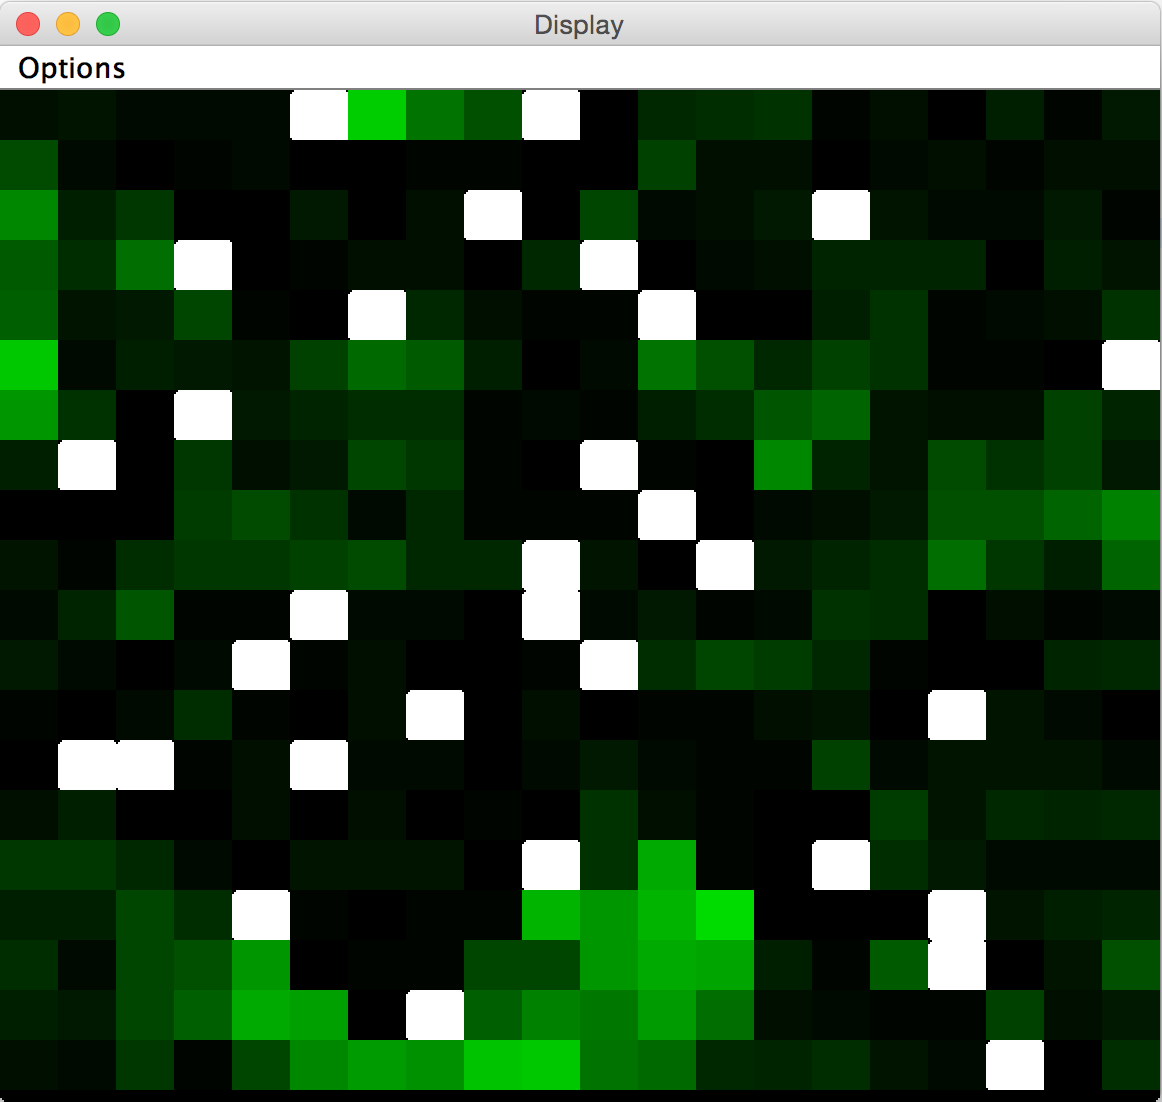
\includegraphics[keepaspectratio=true, width=0.4\textwidth]{rabbits.png}
    \:
    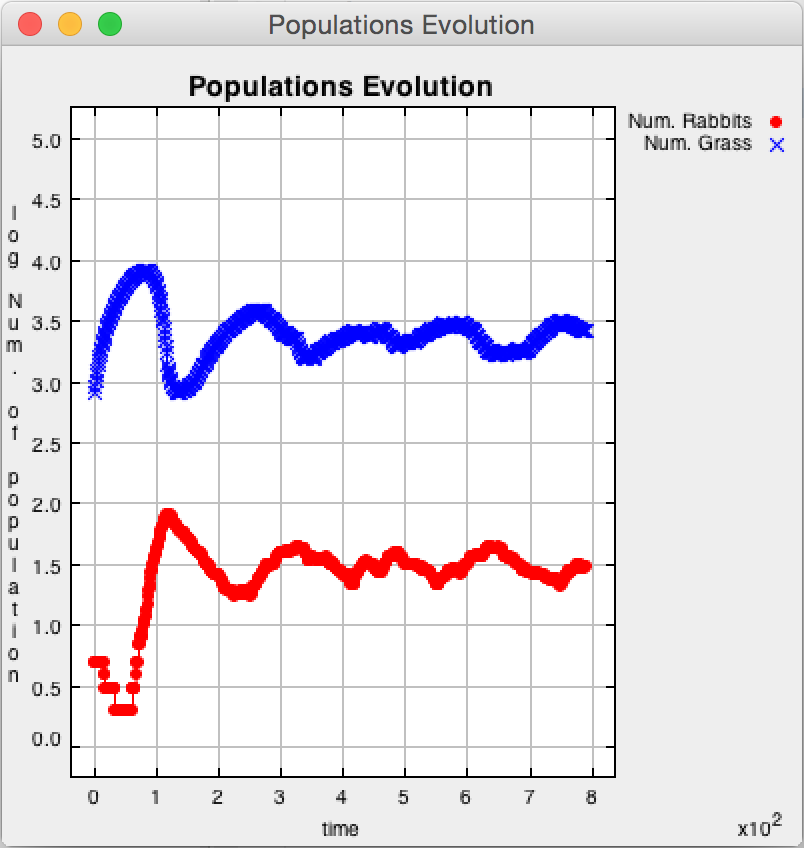
\includegraphics[keepaspectratio=true, width=0.4\textwidth]{graph.png}
\end{titlepage}

%%%%%%%%%%%%%%%%%%%%%%%%%%%%%%%%%%%%%%%%%%%%%%%%%%%%%%%%%%%%%%%%%%%%%%%%%%%%%%%%%%%%%%%%%

%\tableofcontents
%\pagebreak

%%%%%%%%%%%%%%%%%%%%%%%%%%%%%%%%%%%%%%%%%%%%%%%%%%%%%%%%%%%%%%%%%%%%%%%%%%%%%%%%%%%%%%%%%

\section*{Introduction}

In this first lab we implemented a very simple biological model of rabbits living in a discrete, torus world made of grass and nothing else; a relatively peaceful paradise for these little fluffy creatures.

In this simulation, our anosmic rabbits wander around blindly and eat some grass they can find. When they are fat enough, they perform an asexual reproduction and generate an offspring exactly identical to its parent, except for its level of energy and its position on the world since no rabbit is allowed to be on top of another one.

The amount of grass on each discrete cell of the world is also discrete and ranges from 0 (no grass at all) to 500\footnote{which was arbitrarily chosen due to some limitation of RePast's ColorMap class that doesn't have a default colour}. In our universe, the time is governed by a discrete clock. At each clock tick, the total amount of grass of the world is increased by a parametrised amount which is randomly distributed onto the different cells.

Additionally, at each clock tick, every rabbit agent does the following:

\begin{enumerate}
	\item It randomly chooses one of the four direct neighbouring cells and if it is currently rabbit-free, the agent moves there and loses {\fontfamily{courier} MoveEnergyCost} amount of energy; if the destination is currently held by another rabbit, it simply stays where it currently is.
	\item It eats at most MaxEatQuantity amount of the grass available on the current cell it is on.
	\item It consumes a bit of energy (EnergyConsumptionRate) for biological purposes.
	\item If it has enough energy for reproduction (i.e. more than BirthThreshold) and a neighbouring cells is free, then it duplicates itself; the new creature has an amount of energy equals to InitialAgentEnergy and the parent rabbits loses that same amount of energy in order to preserve the total amount of energy.
	\item If the agent has no energy (i.e. less than or equal to zero), the rabbit is considered as dead and removed from the world.
\end{enumerate}

\section*{Simulation Parameters}

In our simulation, the following parameters can be used to tune the system:

\begin{description}
	\item[GridSize] The size of the world; cannot be modified after the simulation was started.
    \item[GrassGrowthRate] The amount of grass being added per clock cycle into the world.
    \item[InitialAmountOfGrass] The overall amount of grass available in the world when the simulation starts.
    \item[InitialRabbits] The number of rabbits already living when the simulation start.
    \item[InitialAgentEnergy] The initial amount of energy a rabbit has when it is given life.
    \item[BirthThreshold] How much energy a rabbit must have to reproduce.
    \item[MaxEatQuantity] The maximal amount of energy a rabbit can eat per clock cycle.
    \item[MoveEnergyCost] The amount of energy a rabbit consumes when it moves to another cell.
    \item[EnergyConsumptionRate] The amount of energy a rabbit loses per clock cycle, in addition to the energy consumed for moving around.
\end{description}

\subparagraph{Graph Evolution}
In our simulation, with default parameters, we see that the populations of grass and rabbits, even if they oscillate, stabilize around a certain mean. We plotted in log scale to have a good vision of the two populations.

\section*{Implementation}

The simulation was implemented using RePast in, hopefully, a usual manner. The model class (RabbitsGrassSimulationModel) manages the different parameters of the simulation, plus a list of rabbit agents (instances of RabbitsGrassSimulationAgent) and a representation of the world capable of being displayed (RabbitsGrassSimulationSpace), in addition of the traditional scheduler. The simulation program can be started using the main function of the MainRabbit class

We used uchicago.src.sim.gui.ColorMap to graphically represent the amount of grass on each cell using RGB colors with this mapping formula:

\[
\mbox{amount of grass } i \mapsto \left( R = 0, G = \min \left\{ 255; i * 5 \right\}, B = 0 \right)
\]


\subparagraph*{How to run the simulation}

In a terminal, simply run ``java -jar salotti-antognini-in.jar``.

\end{document}













